Innerhalb der untersuchten Inventare aus dem Arbeitsgebiet fanden sich keramische Formen, die eindeutig als Vertreter von Stilgruppen des östlich angrenzenden, von \textsc{Wotzka} (1995) untersuchten Inneren Kongobeckens angesprochen werden konnten. Neben einigen Vertretern der Imbonga-Gruppe (Kap.~\ref{sec:IMB-Gr}) entlang des unteren \mbox{Sangha}, fanden sich im Süden des Arbeitsgebietes Gefäßeinheiten (GE) der Stile Bondongo (Kap.~\ref{sec:BDG-Gr}), Mbandaka (Kap.~\ref{sec:MBA-Gr}) und Botendo (Kap.~\ref{sec:BOT-Gr}). Gerade das Verbreitungsgebiet der subrezenten Botendo-Keramik unterstreicht die keramischen Kontakte in der Jüngeren Eisenzeit entlang des südlichen Abschnitts des \mbox{Ubangi} über den Kongo sowie über die Mündungsbereiche von \mbox{Sangha} und \mbox{Likwala}-\mbox{aux}-\mbox{Herbes} hinweg in das Innere Kongobecken.

\subsubsection{Imbonga-Gruppe}\label{sec:IMB-Gr}

Imbonga-Keramik, der älteste Keramikstil im Inneren Kongobecken und zugleich der Startpunkt der als \enquote{Äquator-Co}-Tradition systematisierten Stilabfolge (ebd. 59--68, 221)\footnote{Die interne Variabilität des ursprünglich von \textcite{Eggert.1983} definierten \enquote{Imbonga-Horizonts} wurde von \textcite{Wotzka.1995} in die vier Stilgruppen Imbonga, Bonkake, Ingende und Inganda untergliedert.\label{ftn:AufteilungIMB}}, ließ sich im Arbeitsgebiet lediglich in begrenztem Umfang nachweisen. Dezidierte Komplexe mit Imbonga-Keramik fanden sich lediglich in Mobaka (Fpl.~246, Kat.-Nr.~13) und Mitula (Fpl.~251; Kat.-Nr.~12). Zweifelsfrei der Imbonga-Gruppe zuweisbare Stücke fanden sich überdies nur noch in Gombe (Fpl.~237), knapp südlich der Mündung des \mbox{Ubangi} am linken Kongo-Ufer. Nur unter Vorbehalt ansprechbare GE fanden sich überdies in Bokonongo (Fpl.~250) sowie Ifondo (Fpl.~253) am unteren \mbox{Sangha}. Insgesamt ließen sich vier GE sicher als der Imbonga-Gruppe zugehörig ansprechen, bei sieben weiteren GE war eine Ansprache nur eingeschränkt möglich. Die Funde der Imbonga-Gruppe im nordwestlichen Kongobecken sind äußerst selten und auf den südlichen Abschnitt des Laufes des \mbox{Sangha} beschränkt. Da Grabungen in dieser Region jedoch nur sehr begrenzt durchgeführt wurden, kann das aktuelle Verbreitungsbild lediglich unter Vorbehalt akzeptiert werden.\footnote{In den beiden Grabungen in Bobusa (Kat.-Nr.~6--7) wurden lediglich Schicht-Pakete erfasst, die grundsätzlich eher jüngere Keramik enthielten. Das Gros der bei Grabungen im Inneren Kongobecken erfassten Imbonga-Keramik stammt hingegen aus Grubenbefunden (siehe \textsc{Wotzka} 1995: 302 Kat.-Nr.~1, 326\,f. Kat.-Nr.~17, 349\,f. Kat.-Nr.~35, 353\,f. Kat.-Nr.~37, 385 Kat.-Nr.~42, 359 Kat.-Nr.~44, 382--388 Kat.-Nr.~58--60). Die Fundumstände der im Arbeitsgebiet angetroffenen Imbonga-Keramik (Kat.-Nr. 12--13) legen nahe, dass auch am unteren \mbox{Sangha} Grubeninventare mit Imbonga-Keramik potenziell auffindbar sind. Die hier präsentierten Ergebnisse sollten daher nicht als Beleg für die Nichtexistenz von Imbonga-Keramik gedeutet werden.} Während die Funde aus Mobaka (Kat.-Nr.~13) und Mitula (Kat.-Nr.~12) aus an der Oberfläche erfassten potenziellen Befundzusammenhängen stammen, wurden alle übrigen GE ohne jedweden Kontext als Surveyfunde gemacht. Fragmente von Rändern oder Bodenstücke konnten im untersuchten Material nicht beobachtet werden. Auch die beiden größten GE (Abb.~\ref{fig:IMB_Typentafel}.3,5) waren nur sehr fragmentarisch erhalten.

\begin{figure*}[tb]
	\begin{minipage}[b]{.8\textwidth}
		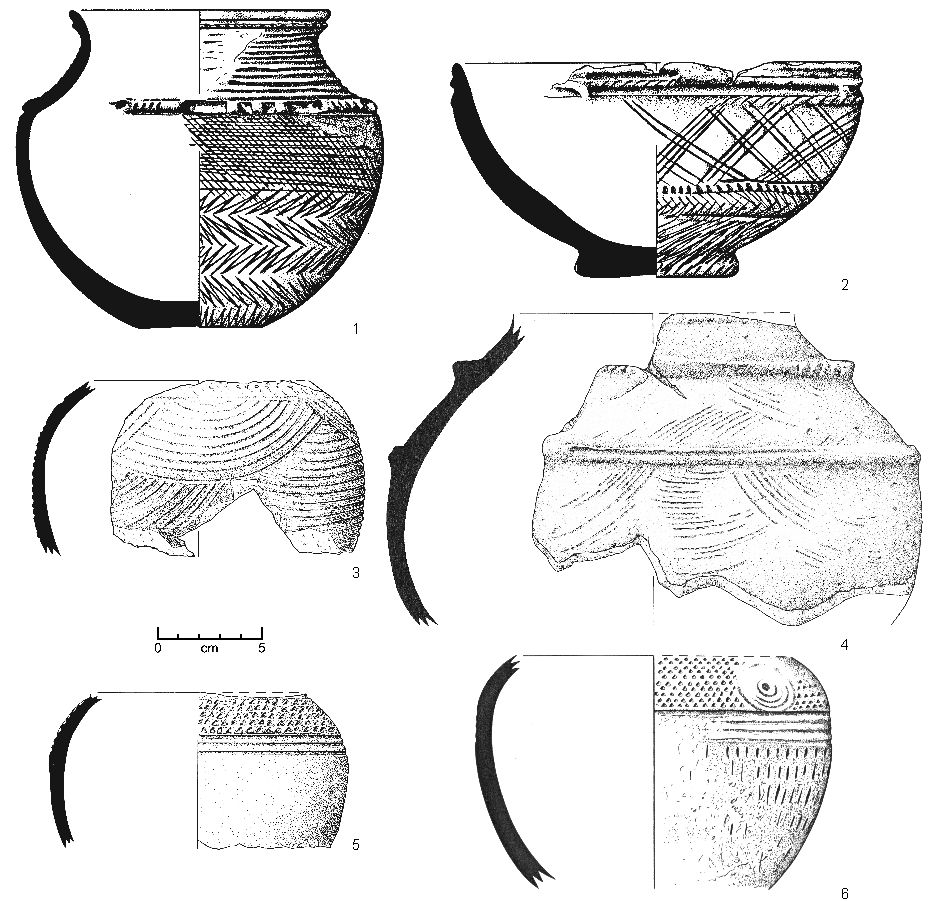
\includegraphics[width=\textwidth]{fig/IMB-Typen.pdf}
	\end{minipage}\hfill
	\begin{minipage}[b]{.2\textwidth}
		\caption{Imbonga-Gruppe: Typvertreter im Arbeitsgebiet (3, 5) sowie Vergleichsfunde aus dem Inneren Kongobecken (1--2, 4, 6).\\1:~\textsc{Wotzka} 1995, 453 Taf.~19.5; 2:~ebd., 453 Taf.~19.6; 3:~Taf.~42.10; 4:~ebd., 441 Taf.~7.7; 5:~Taf.~39.5; 6:~ebd., 453 Taf.~19.10.}
		\label{fig:IMB_Typentafel}
	\end{minipage}
\end{figure*}

\paragraph{Technologische Merkmale}\hspace{-.5em}|\hspace{.5em}%
Alle der Imbonga-Gruppe zugewiesenen GE aus dem Arbeitsgebiet lassen sich dem \textit{Fabric} 1 zuweisen. Im Scherben lassen sich keine nichtplastischen Partikel feststellen und die hellbeige bis weiße Färbung weist auf die Nutzung weißbrennender Tone hin. Anhand der \textit{Fabrics} lassen sich keine Unterscheidungskriterien zwischen der Imbonga-Keramik und der jüngeren, in der \mbox{Sangha}-Region weit verbreiteten Pikunda-Munda-Keramik erarbeiten (Kap.~\ref{sec:PKM-Gr}).

\begin{figure*}[p]
	\centering
	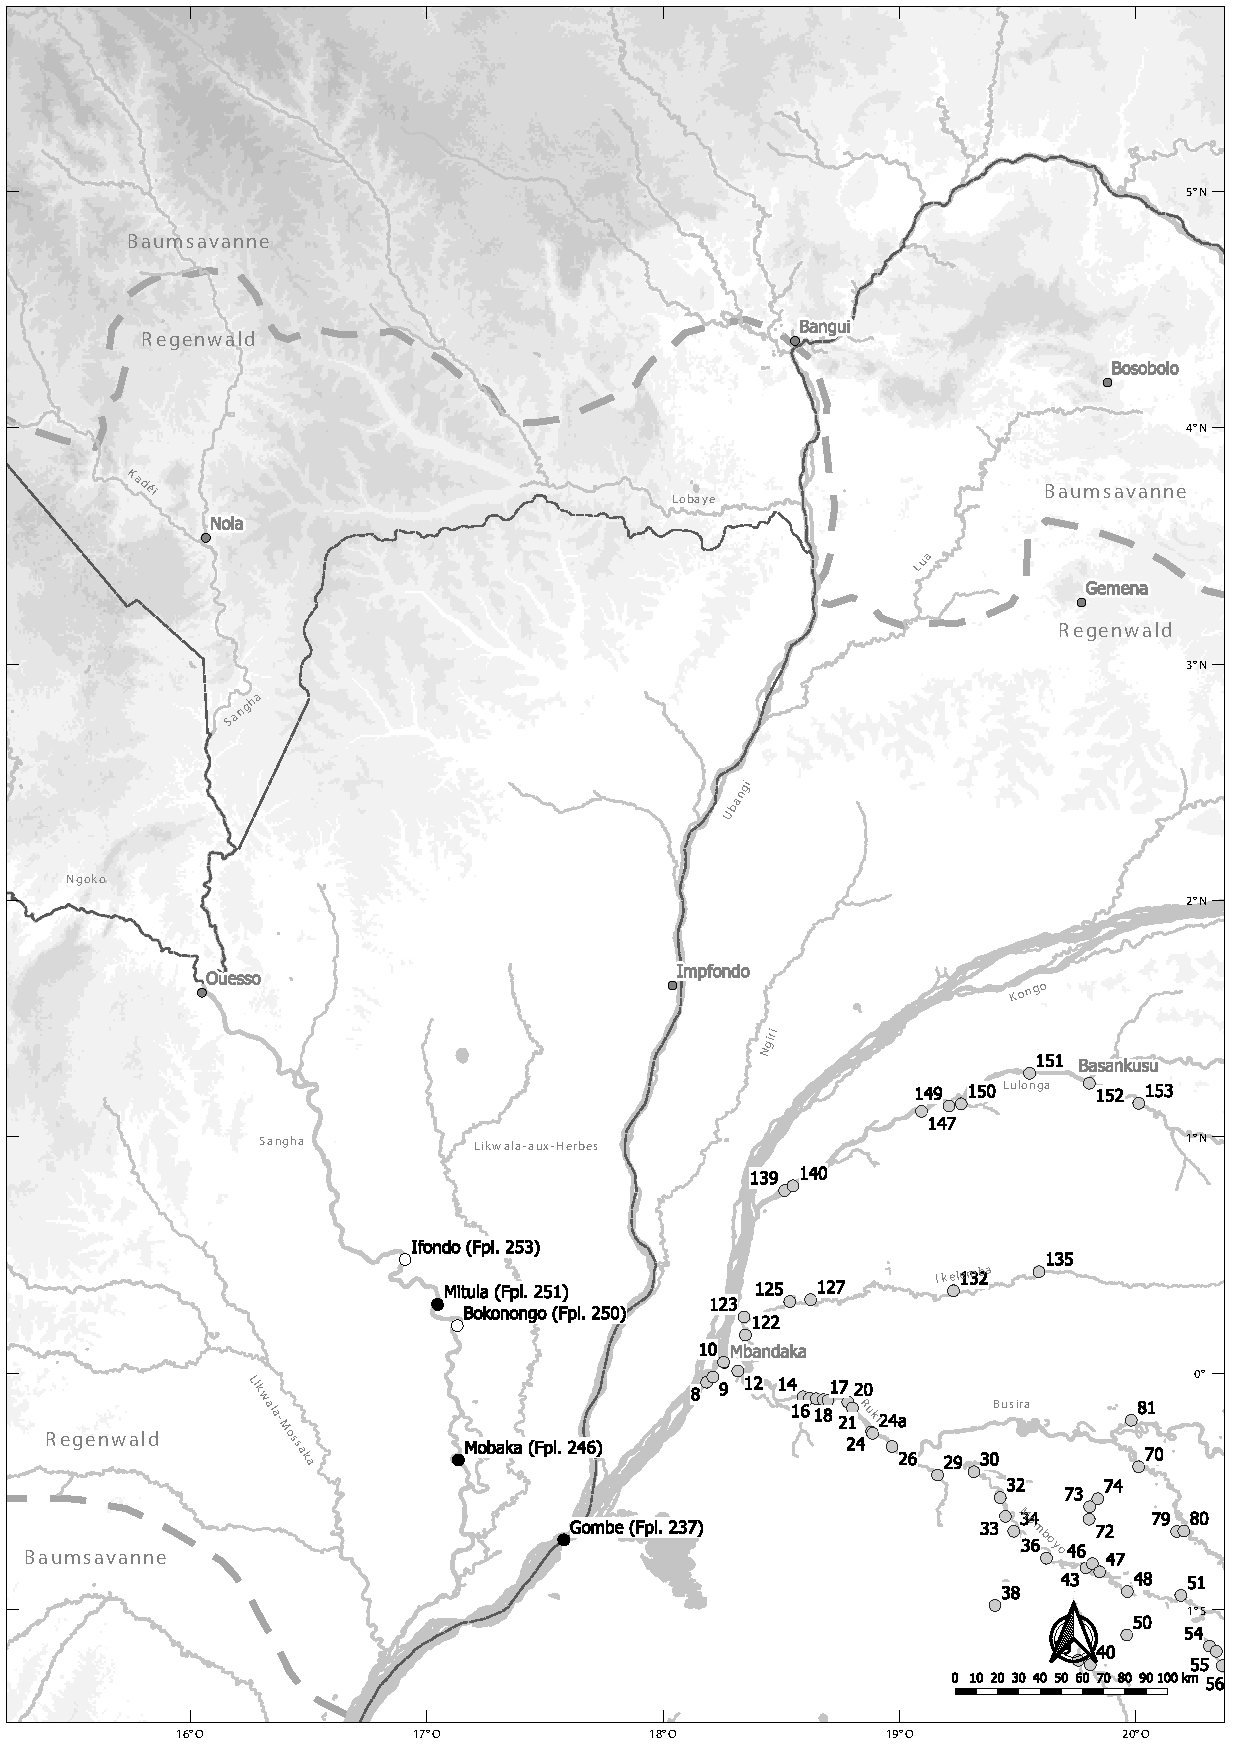
\includegraphics[width=\textwidth]{fig/IMB_Verbreitung.pdf}
	\caption{Imbonga-Gruppe: Verbreitung im Arbeitsgebiet sowie im Inneren Kongobecken \parencite[grau nach][544--545 Karte 2]{Wotzka.1995}.}
	\label{fig:IMB_Verbreitung}
\end{figure*}

\paragraph{Formen}\hspace{-.5em}|\hspace{.5em}%
Das im Arbeitsgebiet erfasste Formenspektrum der Imbonga-Gruppe umfasst keine \textit{klassischen} Vertreter des Imbonga-Stils (Abb.~\ref{fig:IMB_Typentafel}.1--2). Vier der fünf GE aus dem Arbeitsgebiet, bei denen eine Ansprache der Gefäßform möglich war, weisen eine geschweifte Wandung auf (Abb.~\ref{fig:IMB_Typentafel}.3, 5). GE mit den für die Imbonga-Gruppe charakteristischen hohen und ornamental betonten Schulterabsätzen (\textsc{Wotzka} 1995: 60; siehe Abb.~\ref{fig:IMB_Typentafel}.1) ließen sich nicht beobachten. Das Gefäß aus Mitula (Abb.~\ref{fig:IMB_Typentafel}.3; Kat.-Nr.~12) zeigt eine Ornamentik aus bogenförmigen Riefen (Tab.~\ref{tab:Verzierungselemente}: 02.5) und ähnliche Grundform wie ein Gefäß aus der Grabung IYO~81/1 in Iyonda am Kongo (Abb.~\ref{fig:IMB_Typentafel}.4; ebd. 302 Kat.-Nr.~1). Lediglich seine Größe sowie das Fehlen horizontal verlaufender plastischer Leisten unterscheidet es von der GE aus Iyonda. Das Gefäß aus Mobaka (Abb.~\ref{fig:IMB_Typentafel}.5; Kat.-Nr.~13) weist eine fast identische Form und Ornamentik wie ein Gefäße aus der Grabung BKE~81/1 in Bokele am Ruki auf (Abb.~\ref{fig:IMB_Typentafel}.6; ebd. 310--311 Kat.-Nr.~8). Lediglich bei zwei GE waren Bereiche des Gefäßrandes erhalten. In beiden Fällen handelt es sich um einfach ausbiegende Ränder. Böden, die dem Imbonga-Stil entsprechen, liegen nicht vor. 


\paragraph{Verzierungen}\hspace{-.5em}|\hspace{.5em}%
Aufgrund der sehr geringen Anzahl an im Fundgut identifizierten GE des Imbonga-Stils ist auch das beobachtete Spektrum an Verzierungselementen stark ausschnitthaft. Die aufgenommenen Verzierungselemente sind vornehmlich Riefungen (Tab.~\ref{tab:Verzierungselemente}: 02; 53\,\%) sowie Ritzungen (Tab.~\ref{tab:Verzierungselemente}: 01; 18\,\%) und Eindrücke (Tab.~\ref{tab:Verzierungselemente}: 04; 12\,\%). Die für die Imbonga-Keramik des Inneren Kongobeckens charakteristische flächige Wiegebandverzierung der Gefäßunterseiten (Tab.~\ref{tab:Verzierungselemente}: 04.1--2; siehe ebd. 63\,f.) konnte nicht beobachtete werden. Auch die gerillten Ränder, ein weiteres Charakteristikum der Imbonga-Keramik des Inneren Kongobeckens, konnte mangels ansprechbarer Randstücke nicht erfasst werden. Eindeutige Ähnlichkeiten lassen sich ausschließlich zwischen den beiden Gefäßen aus Mitula und Mobaka (Abb.~\ref{fig:IMB_Typentafel}.3, 5) und entsprechenden Vergleichsfunden aus Iyonda sowie Bokele erkennen (Abb.~\ref{fig:IMB_Typentafel}.4, 6). Die Zuweisung der GE aus dem nordwestlichen Kongobecken zur Imbonga-Gruppe ist folglich nur bedingt eindeutig.


\paragraph{Datierung}\hspace{-.5em}|\hspace{.5em}%
Die chronologische Position der Imbonga-Gruppe im Inneren Kongobecken wurde von \textsc{Wotzka} (ebd. 66\,f.) auf Basis von insgesamt neun Radiokohlenstoffdatierungen hinlänglich gut eingegrenzt (Abb.~\ref{fig:14C_InnerCongo_Stylegroups}). Während relativ-chronologische Untersuchungen der Inventare des Inneren Kongobeckens die Imbonga-Gruppe klar an den Beginn der von \textsc{Wotzka} (ebd. 67 Tab.~9) erarbeiteten Stilgruppenentwicklung stellten, wiesen die Radiokohlenstoffdatierungen eine starke Streuung auf.\footnote{Gerade die in den 1980er Jahren in Hannover vorgenommenen Radiokohlenstoffdatierungen streuen in einem so hohen Maße, dass sie von \textsc{Wotzka} (1995: 67 Tab.~9 Nr. 1--2, 9--10) als extreme Ausreißer zurückgewiesen werden \parencite[siehe][]{Geyh.1990}. Auch zwei deutlich zu junge Datierungen aus anderen Labors \parencite[67 Tab.~9 Nr. 11--12]{Wotzka.1995} ließen sich nicht mit der erarbeiteten Chronologie in Einklang bringen. Eine kritische Einschätzung der Hannoveraner Daten findet sich erstmals bei \textcite[132\,f.]{Eggert.1987c}.} Am Ende sieht \textsc{Wotzka} (ebd. 67 Tab.~9 Nr. 3--8) sechs der zwölf absoluten Datierungen, die gemeinsam einen Zeitraum zwischen etwa 400--100 v.~Chr. abdecken, als für die Imbonga-Gruppe repräsentativ an.

Eine Radiokohlenstoffdatierung aus der Füllung des Gefäßes in Mobaka (Kat.-Nr.~13) datiert in das \mbox{8.--1.~Jh.} v.~Chr. (KI-2894), während eine Probe, die unterhalb des Gefäßes in Mitula (Fpl.~12) entnommen wurde, in das 6.--1.~Jh. v.~Chr. (KI-2895) fällt. Die beiden Datierungen decken aufgrund ihrer jeweils hohen Standardfehler einen großen Bereich ab, sind aber grundsätzlich als zeitgleich zu den von \textsc{Wotzka} (ebd. 67 Tab.~9 Nr. 3--8) akzeptierten Datierungen für das Innere Kongobecken anzusehen. 


\paragraph{Verbreitung}\hspace{-.5em}|\hspace{.5em}%
Im nordwestlichen Kongobecken ist Keramik der Imbonga-Gruppe nur äußerst vereinzelt belegt. Die einzigen sicher dieser Stilgruppe zuweisbaren Stücke stammen aus Mobaka (Fpl- 246) und Mitula (Fpl.~251) am unteren \mbox{Sangha} sowie Gombe am Kongo (Fpl.~237). Keines der Stücke stammt aus einer Grabung, obschon die beiden erst genannten Funde zumindest klaren Befunden zugewiesen werden können und individuell datiert sind, sich somit von reinen Oberflächenfunden unterscheiden. Darüber hinaus fand sich nur an drei weiteren Stellen Keramik, die der Imbonga-Gruppe zugerechnet werden kann. Die Fundstelle Gombe (Fpl.~237), die am Kongo liegt, ist räumlich dem Arbeitsgebiet von \textcite{Wotzka.1995} am nächsten. Entlang des \mbox{Sangha} fand sich mögliche Imbonga-Keramik noch in Ifondo (Fpl.~253) -- zugleich die nördlichste der fünf Fundstellen -- und in Bokonongo (Fpl.~250). In beiden Fällen handelt es sich jedoch nur um insgesamt vier fragliche Stücke.\footnote{Die Verbreitung der Imbonga-Gruppe im nordwestlichen Kongobecken ist potenziell vom Naturraum geprägt und wird im Westen durch die Sumpflandschaften des unteren \mbox{Sangha} sowie \mbox{Likwala}-\mbox{aux}-\mbox{Herbes} begrenzt \parencite[siehe][350 Karte 19.1]{Gregoire.2003}.}